\chapter{Theory}

In this chapter, we give a theoretical introduction to the topic dealt with in this thesis. The ultimate goal of this chapter is to introduce and describe a analytical model for subsurface scattering. First, we will give a brief introduction to what light is, and how we physically describe it. Secondly, we will introduce the basic radiometric quantities that will be used throughout the chapter. Then, we will describe how this quantities are related and can be used to describe light-material interaction, using reflectance functions, of which BSSRDF functions are a special case. Finally, we will introduce subsurface scattering and the diffusion approximation, concluding with a description of two BSSRDF functions actually used to describe it, by \cite{Jensen:2001:PMS:383259.383319} and \cite{IMM2013-06646}.

\section{Light and Radiometry}
Light is a form of electromagnetic radiation, a sinusoidal wave that propagates through space. Usually by light we generically refer to \emph{visible light}, the small part of the electromagnetic spectrum the human eye is sensible to. This small window is between 380 nm of the infrared and 770 nm of the ultraviolet, but the precise boundaries vary according to the environment and the observer. Instead explicitly noted, we will use the terms light and visible light interchangeably.

The study of light is usually referred as optics. In computer aided image synthesis, we are interested in representing faithfully how visible light propagates though the scene and how interacts with materials. In addition, we are interested on effects that are noticeable at human scales. So, we are interested for example in subsurface scattering, absorption and emission but not in phenomena like diffraction, interference and quantum effects, that happen on a microscopic scale. 

\begin{figure}[!ht]
\centering
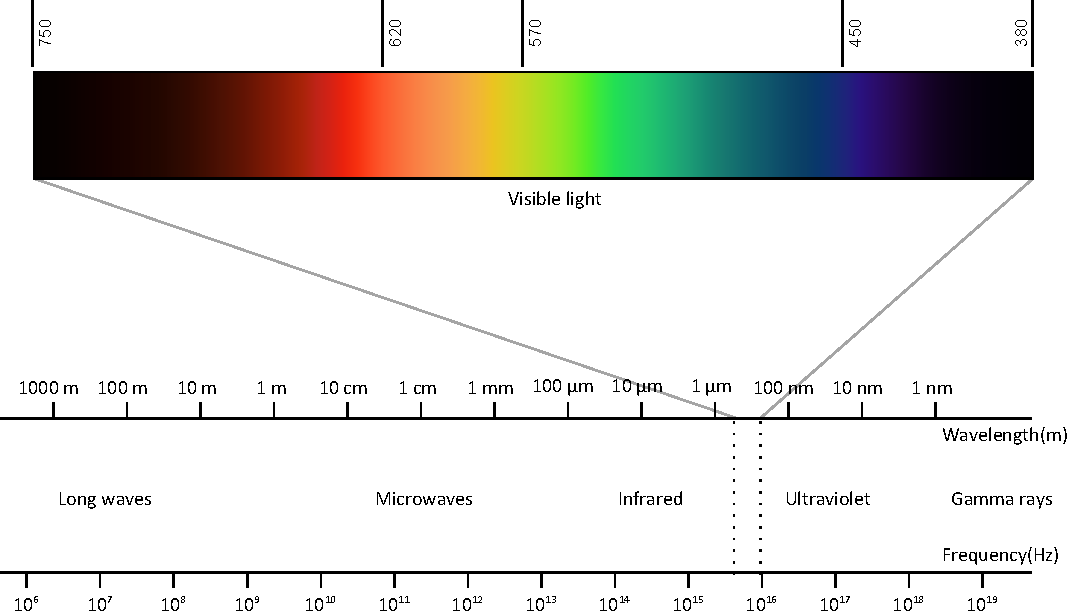
\includegraphics[width=1.0\textwidth]{images/spectrum.pdf}
\caption{The electromagnetic spectrum.}
\label{fig:spectrum}
\end{figure}

The study of the measurement of electromagnetic radiation is called \emph{radiometry}. The energy of light, like all the others forms of energy, is measured in \emph{Joules (J)}, and its power in \emph{Watts (W)}. \emph{Photometry}, on the other hand, measures electromagnetic radiation as it is perceived from the human eye, and limits itself only to the visible spectrum, while radiometry spans all of it. The quantities for energy and power are called respectively \emph{talbot (Cd $\cdot$ s)} and \emph{candela (Cd)}. 

In image synthesis radiometry, is employed, as its quantities are universal and can be easily converted to the photometric ones when necessary. The most important radiometric quantities used in computer graphics are radiant energy, radiant power, radiance, irradiance and intensity.

\section{Radiometric quantities}

\subsection{Radiant flux}
The radiant flux, also known as radiant power, is the most basic quantity in radiometry. It is usually indicated with the letter $\Phi$ and it is measured in joules per seconds ($J/s$) or Watts ($W$). The quantity indicates how much power the light irradiates per unit time. Given its nature, the radiant flux is constant irregardless of the distance from the light source.

\subsection{Radiant energy}
Radiant energy, usually indicated as $Q$, is the energy that the light carries in a certain amount of time. Like all the other SI units for energy, it is measured in joules ($J$). Radiant energy is usually obtained integrating the radiant flux along time:

$$
Q = \int_{\Delta T} \Phi \; dt
$$

Due to the dual nature of the light, the energy carried by the light can be derived both considering the flux of photons as particles, or considering light as a wave. We will not dig further into the topic, because for rendering purposes is not important how we characterize light.

\subsection{Irradiance}

Irradiance, usually defined as $E$, is the radiometric unit that measures the radiant flux per unit area \emph{falling} on a surface. It is measuerd in Watts per square meter ($W/m^2$). It is obtained by further deriving the differential of the radiant flux by the differential area:

$$
E = \frac{d\Phi}{dA}
$$

Irradiance is usually the term using for the incoming power. The converse, i.e. the irradiance leaving a surface, it is usually referred as radiant exitance or radiosity, and indicated with the letter $B$.
 
\subsection{Intensity}
Intensity is often a misused term in the physics community, as it is used for a lot of different measures. Depending on the community, intensity may refer to irradiance or even to radiance (see following section). We will refer to intensity as it is generally interpreted by the optics community, i.e. radiant intensity. It is defined as the differential radiant flux per differential solid angle:

$$
I(\vec{\omega}) = \frac{d \Phi}{d \omega}
$$

Intensity is measured in Watts / steradian ($W/sr$) and it is indicated with the letter $I$.

\subsection{Radiance}
Radiance is the most important quantity in image synthesis. It is defined precisely as the differential flux per solid angle per projected surface area, and it is measured in Watt per steradian per square meter ($W / (sr \cdot m^2)$).

$$
L(\vec{\omega}) = \frac{d^2 \Phi}{d\omega dA \cos \theta}
$$

Where $\theta$ is the angle between the surface normal and the incoming ray of light. Radiance is important in image synthesis because it is the natural quantity to associate with a ray of light (as it remains constant) and because is the quantity the human eye is actually sensible to. For a discussion on why radiance is related to the sensitivity of sensors and the human eye, see X.

All the other radiometric quantities can be derived from radiance:

\begin{equation*}
\begin{split}
E &= \int_{2\pi} L_i(\vec{\omega}) \cos\theta \; d\omega \\
I(\vec{\omega}) &= \int_A L(\vec{\omega}) \cos\theta \; dA \\
\Phi &= \int_A \int_{2\pi} L(\vec{\omega}) \cos\theta \; d\omega dA
\end{split}
\end{equation*}

\subsection{Radiometric quantities for simple lights}
To help with the formulas used later in the report, we derive the above mentioned radiometric quantities for the two simplest types of light, i.e. directional and point lights.
\begin{itemize}
	\item \textit{Directional lights} simulate very distant light sources, in which all the rays of light are parallel (i.e. the sun). They are represented by a direction $\vec{\omega}_l$ and a constant radiance value, $L$. 
	\item \textit{Point light} simulate lights closer to the observer. Isotropic point lights are represented by a position of the light $\mathbf{x}_l$ and a constant intensity $I$. Point lights have a fall off that depends on the inverse square law, i.e. the radiance diminishes with the square of the distance.
\end{itemize}

Table \ref{table:radio} shows different radiometric quantities evaluated for point and directional lights, for a surface point $\mathbf{x}$ with surface normal $\vec{n}$. 

\renewcommand{\arraystretch}{1.8}
\begin{table}[!ht]
    \centering
    \begin{tabularx}{0.95\textwidth}{|X|X|X|}
    \hline
    Quantity   & Directional light & Point light \\ \hline
    Cosine term       & $\cos\theta = \vec{n} \cdot \vec{\omega}_l$ & $\cos\theta = \frac{(\mathbf{x} - \mathbf{x}_l) \cdot \vec{n}}{|\mathbf{x} - \mathbf{x}_l|}$     \\ \hline

    $\Phi(\mathbf{x})$ Flux       & $\infty$                  & $4 \pi I$           \\ \hline
    $E(\mathbf{x})$ Irradiance & $L \cos\theta $                 & $I \frac{\cos\theta}{|\mathbf{x}_l - \mathbf{x}|^2}$          \\ \hline
    $I(\mathbf{x},\vec{\omega})$ Intensity  & $\infty$                 & $I$           \\ \hline
    $L(\mathbf{x},\vec{\omega})$ Radiance   & $L$               & $\frac{I}{|\mathbf{x}_l - \mathbf{x}|^2}$           \\ \hline
    \end{tabularx}
\caption{Different radiometric values for simple light sources.}
\label{table:radio}
\end{table}

\section{Reflectance Functions}
 
After introducing the basic radiometric quantities, we still lack a way to describe light material interaction. More precisely, we need a way to relate the incoming and the outgoing radiance on a point of a chosen surface. As we have already discussed before, we use radiance since is the radiometric quantity that is directly proportional to what the human eye measures. 

\subsection{BRDF functions}

One of the possible way to describe light-material interaction is by using a BDRF function, acronym for \emph{Bidirectional Reflectance Distribution Function}. The BRDF function $f(\mathbf{x}, \vec{\omega}_i, \vec{\omega}_o)$ is defined on one point $\mathbf{x}$ of the surface as the differential ratio between the exiting radiance and the incoming irradiance:

\begin{equation}
f(\mathbf{x}, \vec{\omega}_i, \vec{\omega}_o) = \frac{d L_o(\mathbf{x}, \vec{\omega}_o)}{d E_i(\mathbf{x}, \vec{\omega}_i)} = \frac{d L_o(\mathbf{x}, \vec{\omega}_o)}{L_i(\mathbf{x}, \vec{\omega}_i) \cos\theta_i d \vec{\omega}_i}
\label{eq:brdf}
\end{equation}

The BRDF states that the incoming and the outgoing radiance are proportional, so that the energy hitting the material at the point $\mathbf{x}$ is proportional to the energy coming out from the point. The BRDF function is generically reciprocal for the Hemholtz reciprocity principle ( $f(\mathbf{x}, \vec{\omega}_i, \vec{\omega}_o) = f(\mathbf{x}, \vec{\omega}_o, \vec{\omega}_i)$), and anisotropic (if the surface changes orientation and $\vec{\omega}_i$ and $\vec{\omega}_o$ are the same, the resulting BRDFs are different). In addition, it is positive( $f(\mathbf{x}, \vec{\omega}_o, \vec{\omega}_i) \ge 0$), and conserves energy, so that the energy of the outgoing ray is no grater that the one of the incoming one ($\int_{2\pi}  f(\mathbf{x}, \vec{\omega}_o, \vec{\omega}_i) \cos\theta_o d\vec{\omega}_o \le 1$).

By inverting equation \ref{eq:brdf}, we obtain the so-called \emph{reflectance equation}:

$$
L_o(\mathbf{x}, \vec{\omega}_o) = \int_{2\pi} f(\mathbf{x}, \vec{\omega}_i, \vec{\omega}_o) L_i(\mathbf{x}, \vec{\omega}_i) \cos\theta_i d\vec{\omega}_i
$$

That later we will extend to obtain the rendering equation. The BRDF function has some limitations, being not able to account for all phenomena. For example, with a BRDF it is not possible to account for subsurface scattering phenomena, because it assumes the light enters and leaves the material in the same point. To model these phenomena, more complicated functions are needed, like the BSSRDF function described later in this chapter. 

\subsection{Examples of BRDF functions}

There are many examples of BRDF functions in literature. In this section, we will introduce three of the simplest ones: for a more exhaustive description of BRDF functions, refer to X. The three BRDFs are the lambertian or diffuse BRDF, the specular or mirror BRDF and the Blinn-Phong BRDF.

\subsubsection{Lambertian BRDF}

In the lambertian BRDF, the incoming radiance is distributed equally in all directions, regardless of the incoming directions. To do this, the BRDF must be constant:

$$
f(\mathbf{x}, \vec{\omega}_i, \vec{\omega}_o) = k_d
$$

We can check that then the radiance is scattered equally in all directions by simple integration:

\begin{equation*}
\begin{split}
L_o(\mathbf{x}, \vec{\omega}_o) &= \int_{2\pi} f_d L_i(\mathbf{x}, \vec{\omega}_i) \cos\theta_i d\vec{\omega}_i \\
L_o(\mathbf{x}, \vec{\omega}_o) &= k_d \int_{2\pi} L_i(\mathbf{x}, \vec{\omega}_i) \cos\theta_i d\vec{\omega}_i \\
L_o(\mathbf{x}, \vec{\omega}_o) &= k_d \; E(\mathbf{x}) \\
\end{split}
\end{equation*}

The lambertian model is an ideal model, so very few material exhibit a lambertian diffusion, like unfinished wood or spectralon, a synthetic material created in order to have a lambertian diffusion. 

\subsubsection{Mirror BRDF}

Another simple kind of BRDF is the perfectly specular BRDF, or mirror BRDF. In this function, all the incoming radiance from one direction $\vec{\omega}_i$ is completely diffused into the reflected direction $\vec{\omega}_r$, defined as $\vec{\omega}_r = \vec{\omega}_i - 2 (\vec{\omega}_i \cdot \vec{n}) \vec{n}$. The resulting BRDF is defined as follows:

$$
f(\mathbf{x}, \vec{\omega}_i, \vec{\omega}_o) = \frac{\delta(\vec{\omega}_o - \vec{\omega}_r)}{\cos\theta_i} 
$$

The function $\delta(\vec{\omega})$ is a hemispheric delta function. Once integrated over a hemisphere, the function evaluates to one only for the vector $\vec{\omega} = \mathbf{0}$. Putting the BRDF into the reflectance equation gives the following outgoing radiance:

\begin{equation*}
L_o(\mathbf{x}, \vec{\omega}_o) = \begin{cases}
L_i(\mathbf{x}, \vec{\omega}_i)  &\text{if $\vec{\omega}_o = \vec{\omega}_r$}\\
0 &\text{otherwise}
\end{cases}
\end{equation*}

that is the expected result, as all the radiance is diffused into the direction $\vec{\omega}_r$.

\subsubsection{Glossy BRDFs}

As we can see from real life experience, rarely objects are completely diffuse or completely specular. These two models are idealized models, that represent an ideal case. So, to create a realistic BRDF model, we often need to combine the two terms and add an additional one, called glossy reflection. This term is often needed to model the behaviour of the surface more realistically, especially at grazing angles.

The most used BRDF model used to model glossy reflections is based on microfacet theory. In this theory, the surface of an objecct is modeled as composed of small mirrors. In one of its classical formulation, the BRDF is represented as:

$$
f(\mathbf{x}, \vec{\omega}_i, \vec{\omega}_o) = \frac{D G F}{4 \cos\theta_r \cos\theta_i} = \frac{G F}{4} \frac{(\vec{n}\cdot\vec{h})^s}{(\vec{n}\cdot\vec{r})(\vec{n}\cdot\vec{\omega}_i)}
$$

$D$ regulates how microfacets are distributed, and it is often modeled as $(\vec{n}\cdot\vec{h})^s$, where $\vec{h}$ is the half vector between the eye and the light, and $s$ is an attenuation parameter. $G$ accounts for the object self shadowing, while $F$ is the Fresnel reflection term (more details in section Y).	$\vec{r}$ is the reflection vector as defined in the previous section. See figure Z on how the vectors for the glossy reflection - $\vec{n}$, $\vec{h}$ and $\vec{r}$ - are defined.

Various alternative definitions exist for the $D$ and $G$ function, varying among the literature. Other glossy models exist, not based on microfacet theory. 

\subsection{The rendering equation}

Given the reflectance equation, it is possible to generalize it in order to model all the lighting in an environment. In fact, this form of the reflectance equation does not account for two factors. 

The first factor are emissive surfaces. We need to add an emissive radiance term $L_e(\mathbf{x}, \vec{\omega})$ that models how much radiance is a point on a surface emitting in a certain directions. This is useful to model lights as any other surface in the scene. Note that point lights have a singularity: they emit infinite radiance on the point they are placed.

The second factor is that the reflectance equation accounts only for direct illumination. In general, we want to model global illumination, i.e. to include also light that bounced onto another surface before reaching the current surface. To model this, we can replace the $L_i$ term in the reflectance equation with another term $L_r$ that accounts for reflected radiance. This term can be usually modeled as the product of the radiance of the light plus a visibility function $V(\mathbf{x})$.

Accounting for all the described factors, we reach the true form of the rendering equation:

$$
L_o(\mathbf{x}, \vec{\omega}_o) = L_e(\mathbf{x}, \vec{\omega}) + \int_{2\pi} f(\mathbf{x}, \vec{\omega}_i, \vec{\omega}_o) L_i(\mathbf{x}, \vec{\omega}_i) V(\mathbf{x}) \cos\theta_i d\vec{\omega}_i
$$

This form of the rendering equation is still not completely general, since it is based on a BRDF, so no subsurface scattering effects or wavelength-changing effects (like iridescence) are impossible to model. We will extend the rendering equation in order to account for these phenomena later on in this chapter.

\subsection{Fresnel equations}

Until now, on the considered models, we did consider only the reflected part of the radiance. When a beam of light coming from direction $\vec{\omega}_i$ hits a surface, only part of the incoming radiance gets reflected, while another part gets refracted into the material. As we can see from the setup from figure Z, we obtain the two vectors $\vec{\omega}_r$ and $\vec{\omega}_t$, the reflected and refracted vector, defined as follows:

\begin{equation*}
\begin{split}
\vec{\omega}_r &= \vec{\omega}_i - 2 (\vec{\omega}_i \cdot \vec{n}) \vec{n} \\
\vec{\omega}_t &= \eta ((\vec{\omega}_i \cdot \vec{n}) \vec{n} - \vec{\omega}_i) - \vec{n} \sqrt{1 - \eta^2 (1 - (\vec{\omega}_i \cdot \vec{n}) ^ 2)}
\end{split}
\end{equation*}

Where $\eta = \frac{n_1}{n_2}$ is the relative index of refraction of the material. With this setup, we can use a solution to Maxwell's equations for wave propagation to describe how light spreads between reflected and refracted directions. what we obtain are called \emph{Fresnel coefficients}. The coefficients are different according to the polarization of the incoming light, so there are two for the reflection ($R_s$, $R_p$) and two for transmission ($T_s$, $T_p$). The coefficients relate the incoming and outgoing power of the light, and by differentiation, the radiance as well.

\begin{equation*}
\begin{split}
R_s = \left|\frac{n_1 \cdot \cos\theta_i - n_2 \cdot \cos\theta_t} {n_1 \cdot \cos\theta_i + n_2 \cdot \cos\theta_t}\right|^2 \;\;\;&\;\;\; R_p = \left|\frac{n_1 \cdot \cos\theta_t - n_2 \cdot \cos\theta_i} {n_1 \cdot \cos\theta_t + n_2 \cdot \cos\theta_i}\right|^2\\
T_s = \frac{n_2 \cdot \cos\theta_t}{n_1 \cdot \cos\theta_i} \left|\frac{2 n_1 \cdot \cos\theta_i}{n_1 \cdot \cos\theta_i + n_2 \cdot \cos\theta_t}\right|^2 \;\;\;&\;\;\; T_p = \frac{n_2 \cdot \cos\theta_t}{n_1 \cdot \cos\theta_i}  \left|\frac{2 n_1 \cdot \cos\theta_i}{n_1 \cdot \cos\theta_t + n_2 \cdot \cos\theta_i}\right|^2
\end{split}
\end{equation*}

In most computer graphics applications, we assume that the two polarizations are equally mixed. So, we will use the coefficient $R = \frac{R_s + R_p}{2}$ and $T = \frac{T_s + T_p}{2}$ in our calculations. Note that $R + T = 1$, so the overall energy is conserved.

%vec3 refract2(vec3 inv, vec3 n, float n1, float n2)
%{
    %float eta = n1/n2;
    %float c = dot(inv, n);
    %return eta * (c * n - inv) - n * sqrt(max(0.0f,1 - eta * eta * (1 - c * c)));
%}


\section{Light transport and subsurface scattering}
\subsection{BSSRDF functions and generalized rendering equation}
\subsection{Scattering parameters}
 emission, absorption, scattering and phase functions
\subsection{Standard dipole model}
\subsection{Directional dipole model}
